% The seven bridges of Königsberg
% Author : Alain Matthes
% Encoding : UTF8
% Engine : PDFLaTeX
\documentclass[]{article}
\usepackage[utf8]{inputenc} 
\usepackage{fullpage}
\usepackage{fourier}
\usepackage{tikz}
\usetikzlibrary{arrows,shapes,positioning}
               

\thispagestyle{empty}
\begin{document}

  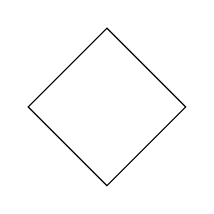
\begin{tikzpicture}
\draw (1,0) -- (0,1) -- (-1,0) -- (0,-1) -- cycle;
\end{tikzpicture}

foobar
foobar

foobar
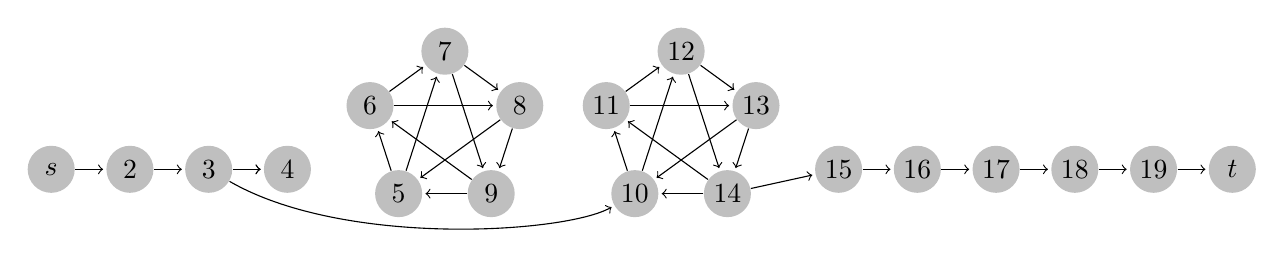
\begin{tikzpicture}[shorten >=1pt,->]
  \tikzstyle{vertex}=[circle,fill=black!25,minimum size=17pt,inner sep=0pt]

  \foreach \name/\x in {s/1, 2/2, 3/3, 4/4, 15/11, 
                        16/12, 17/13, 18/14, 19/15, t/16}
    \node[vertex] (G-\name) at (\x,0) {$\name$};

  \foreach \name/\angle/\text in {P-1/234/5, P-2/162/6, 
                                  P-3/90/7, P-4/18/8, P-5/-54/9}
    \node[vertex,xshift=6cm,yshift=.5cm] (\name) at (\angle:1cm) {$\text$};

  \foreach \name/\angle/\text in {Q-1/234/10, Q-2/162/11, 
                                  Q-3/90/12, Q-4/18/13, Q-5/-54/14}
    \node[vertex,xshift=9cm,yshift=.5cm] (\name) at (\angle:1cm) {$\text$};

  \foreach \from/\to in {s/2,2/3,3/4,3/4,15/16,16/17,17/18,18/19,19/t}
    \draw (G-\from) -- (G-\to);

  \foreach \from/\to in {1/2,2/3,3/4,4/5,5/1,1/3,2/4,3/5,4/1,5/2}
    { \draw (P-\from) -- (P-\to); \draw (Q-\from) -- (Q-\to); }

  \draw (G-3) .. controls +(-30:2cm) and +(-150:1cm) .. (Q-1);
  \draw (Q-5) -- (G-15);
\end{tikzpicture}


  The Seven Bridges of Knigsberg is a famous historical problem in mathematics. Its negative resolution by Leonhard Euler in 1735 laid the foundations of graph theory and presaged the idea of topology.
  
  Abstract graph corresponding to bridges of Knigsberg 
  
\begin{center}
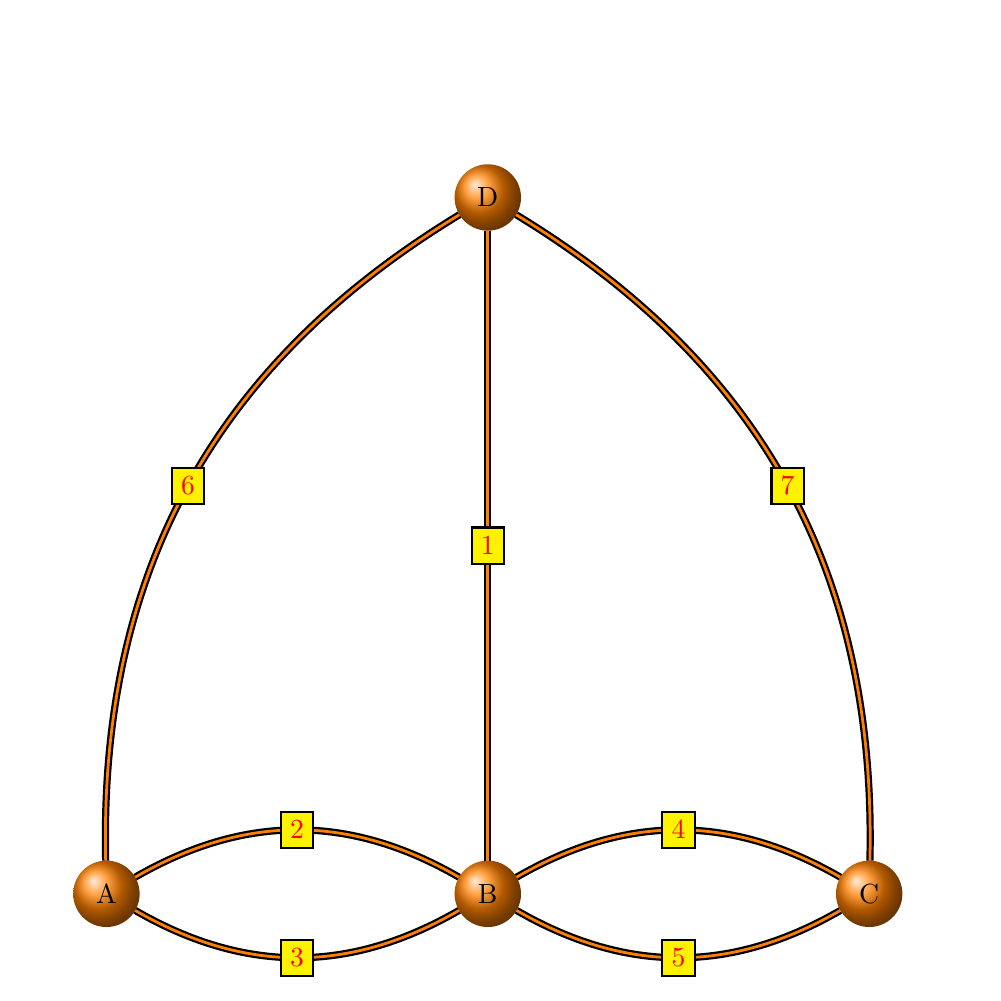
\begin{tikzpicture}[node distance   = 4 cm]
  \useasboundingbox (-1,-1) rectangle (11,11); 
  \tikzset{VertexStyle/.style = {shape          = circle,
                                 ball color     = orange,
                                 text           = black,
                                 inner sep      = 2pt,
                                 outer sep      = 0pt,
                                 minimum size   = 24 pt}}
  \tikzset{EdgeStyle/.style   = {thick,
                                 double          = orange,
                                 double distance = 1pt}}
  \tikzset{LabelStyle/.style =   {draw,
                                  fill           = yellow,
                                  text           = red}}
     \node[VertexStyle](A){A};
     \node[VertexStyle,right=of A](B){B};
     \node[VertexStyle,right=of B](C){C};
     \node[VertexStyle,above= 8 cm of B](D){D};     
     \draw[EdgeStyle](B) to node[LabelStyle]{1} (D) ;
     \tikzset{EdgeStyle/.append style = {bend left}}
     \draw[EdgeStyle](A) to node[LabelStyle]{2} (B);
     \draw[EdgeStyle](B) to node[LabelStyle]{3} (A);
     \draw[EdgeStyle](B) to node[LabelStyle]{4} (C);
     \draw[EdgeStyle](C) to node[LabelStyle]{5} (B);
     \draw[EdgeStyle](A) to node[LabelStyle]{6} (D);
     \draw[EdgeStyle](D) to node[LabelStyle]{7} (C);

  \end{tikzpicture}
\end{center}
\end{document}
